\documentclass[11pt, letterpaper,titlepage,oneside]{article}
%One inch margins
\usepackage[margin=1in]{geometry}
%Header/footer stuff
\usepackage{titlesec}
\usepackage{fancyhdr}
\fancyhf{}
\rfoot{\thepage}
\renewcommand{\headrulewidth}{0pt}
\pagestyle{fancy}
%paragraph indentation
\usepackage[parfill]{parskip}
\parskip = \baselineskip
\setlength{\parindent}{0in}
%Graphic Stuff
\usepackage{xcolor,graphicx}
\usepackage{float}
%Math tools
\usepackage{amsmath}
\usepackage{mathptmx}
\usepackage{lipsum}
%One and half spacing
\usepackage{setspace}
\onehalfspacing
%End one and a half spacing
%Algorithm
\usepackage{algorithm}
\usepackage{algorithmic}
\renewcommand{\arraystretch}{1}
% Caption Formatting
\usepackage{caption}
\captionsetup[figure]{labelsep=period}
\captionsetup[table]{labelsep=newline, justification=centering}
\renewcommand{\tablename}{TABLE}
\renewcommand{\thetable}{\Roman{table}}
\usepackage{fixltx2e}
%Title Page
\newcommand{\titles}{\LARGE \textbf{Load Balancing Unstructured Meshes for Massively Parallel Transport Sweeps in PDT}}
\newcommand{\authors}{\normalsize Tarek Ghaddar \\ Chair: Dr. Jean Ragusa \\ Committee: Dr. Jim Morel, Dr. Bojan Popov}
\newcommand{\department}{\normalsize Nuclear Engineering Department}
\newcommand{\university}{\normalsize Texas A\&M University}
\newcommand{\locations}{\normalsize College Station, TX, 77843-3133}
%Script font
\usepackage[mathscr]{euscript}
\renewcommand{\thesection}{\Roman{section}.}
\renewcommand{\thesubsection}{\thesection\Alph{subsection}.}
\renewcommand{\thesubsubsection}{\thesection\Alph{subsection}.\arabic{subsubsection}}
%Include a pdf file
\usepackage{pdfpages}
%Using the .bib file
\usepackage[superscript,biblabel]{cite}
%Changing spacing in itemized lists
\usepackage{enumitem}
\setlist{nosep}

\newcommand{\tcr}[1]{\textcolor{red}{#1}}
\newcommand{\vr}{\vec{r}}
\newcommand{\vo}{\vec{\Omega}}

%%%%%%%%%%%%%%%%%%%%%%%%%%%%%%%%%%%%%%%%%%%%%%%%%%%%%%%%%%%%%%%%%%%%%
\begin{document}
%%%%%%%%%%%%%%%%%%%%%%%%%%%%%%%%%%%%%%%%%%%%%%%%%%%%%%%%%%%%%%%%%%%%%

\begin{titlepage}
\begin{center}
  \vspace*{3.81 cm}
  \titles\\
  \vspace*{4.445cm}
  \authors \\
  \vspace*{2.54cm} 
  \department \\
  \university \\
  \locations \\
\end{center}
\end{titlepage}


%%%%%%%%%%%%%%%%%%%%%%%%%%%%%%%%%%%%%%%%%%%%%%%%%%%%%%%%%%%%%%%%%%%%%
%%%%%%%%%%%%%%%%%%%%%%%%%%%%%%%%%%%%%%%%%%%%%%%%%%%%%%%%%%%%%%%%%%%%%
\section{Introduction}
%%%%%%%%%%%%%%%%%%%%%%%%%%%%%%%%%%%%%%%%%%%%%%%%%%%%%%%%%%%%%%%%%%%%%
%%%%%%%%%%%%%%%%%%%%%%%%%%%%%%%%%%%%%%%%%%%%%%%%%%%%%%%%%%%%%%%%%%%%%

\tcr{don't talk about PDT here\\
TE first, one-speed, non SN form keep the integro-differential aspects\\
then introduce SI, ell, q =rhs= total src = scat from prev iter+ext\\
then introduce directions, m\\
discont approx, Reed LANL 1973}

The steady-state neutron transport equation describes the behavior of neutrons in a medium, and is given by Eq. \ref{continuous transport}:
\begin{equation}
\vo \cdot \vec \nabla \psi(\vr,E,\vo) +\Sigma_t(\vr,E) \psi(\vr,E,\vo)  =
\int_{0}^{\infty}dE' \int_{4\pi}d\Omega' \Sigma_s(E'\to E, \Omega'\to\Omega)\psi(\vr,E',\vo') 
+ S_{ext}(\vr,E,\vo) ,
\label{continuous transport}
\end{equation}
where $\vec{\Omega}_{m}\cdot \vec\nabla\psi$ is the leakage term and $\Sigma_t\psi$ is the total collision term (absorption and outscatter). These are the loss terms of the neutron transport equation. The right hand side of Eq. \ref{continuous transport} represent the gain terms, where $S_{ext}$ is the external source of neutrons and $\int_{0}^{\infty}dE'\int_{4\pi}d\Omega'\Sigma_s(E'\to E, \Omega'\to\Omega)\psi(\vr,E',\vo')$ is the inscatter term, which represents all neutrons scattering from energy $E'$ and direction $\vo'$ into energy $dE$ about $E$ and $d\Omega$ about direction $\vo$.
\tcr{in your version you called $\Omega_i$ an energy. Why?}

Often, we like to solve the transport equation just for one group and one direction of neutrons \tcr{no}. 
This results in the inscatter term dropping from the equation \tcr{you need to spend some time on my sweep tasks and report your progress and ask questions, what you are saying here is very incorrect}, as we've \tcr{do not use contraction} made the assumption that all neutrons will exist at one energy. As a result, we only care about neutrons that will no longer be at that energy. Thus our only neutron gain is from the external source and from fission \tcr{I removed fission. It does not contribute to the clarity of the document, nor is it relevant to the problem at hand}. \tcr{that was a long and convoluted sentence to arrive at the multigroup expression. Think this over} However, we also often wish to solve for several groups of neutrons, and Eq. \ref{multigroup} is used for this multigroup approach:
\begin{equation}
\vec{\Omega}\cdot \vec\nabla\psi_g + \Sigma_{t,g}\psi_g = S_g + \sum_{g^{\prime}}\Sigma_{s,g^{\prime}\to g}\psi_{g},
\label{multigroup}
\end{equation}
\tcr{explain how an approximation on the energy variable removes the angular integral...}
where for convenience, we have combined the fission term and external source term into one source term, $S_g$. The subscript $g$ represents the current energy group. The last term on the right hand side we see represents the summation of neutrons scattered in from all groups $g^{\prime}$ into current group $g$.

All that's left is to add in the consideration of inscatter from neutrons traveling in different directions, shown in Eq. \ref{discretetransport}:
\begin{equation}
\vec{\Omega}_{m}\cdot \vec\nabla \psi^{(l+1)}_{m,g} + \Sigma_{t,g}\psi_{m,g}^{(l+1)} = S_{m,g}^{(l)} + \sum_{g^\prime}\sum_{m^{\prime}}\omega_m\Sigma_{s,g^{\prime}\to g,m^\prime\to m}\psi_{m^\prime g^\prime}^{(l)},
\label{discretetransport}
\end{equation}
\tcr{I would not introduce the anglar discretization, index m, at the same time as the iterative index l; it's confusing}
where we have added the subscript $m$ and an extra summation of all directions $m^{\prime}$ scattering into direction $m$. Also shown is the superscript $l$, which introduces the concept of source iteration. Source iteration is a fundamental concept of the transport sweeps. The total source term is calculated, a sweep is performed, and is repeated until the \tcr{the what? noun is missing}$\psi^{(l+1)}-\psi^{(l)}$ converges to a specified tolerance.

\tcr{after all of this, a bit of simplicity would be refreshing. for one direction m, the TE, accounting for the total source $q_m$ in direction m, defined as the sum of the external source in that direction and the contribution of the collision source computed with the previous scalar flux, is simply}
\[
\vo_m \cdot \nabla \psi_m + \Sigma_t \psi_m = q_m
\]
\tcr{ now that the energy and angle variables have been treated, it is time to discuss the spatial discretization. Its discontinuous nature, due to the use of finite differences or discontinuous finite elements WITH upwind is the reason why the above equation can be solved one spatial cell at a time ....}

Transport sweeps on unstructured meshes would not be possible without the work on the discontinuous finite element approximation performed by Reed and Willis at Los Alamos and the University of California\cite{Reed}. \tcr{pompous}
\tcr{some graphics explaining sweeps on structured and unstructured meshes are welcome here}

\tcr{you will be using the term graph later on, here is a good place to make the connection between a sweep and a graph}


\tcr{brief intro to PDT, mostly the parallel aspects}

PDT is Texas A\&M University's massively parallel deterministic transport code. It is capable of multi-group simulations, and employs discrete ordinates for angular discretization. Types of simulations include steady-state, time-dependent, criticality, and depletion simulations. It solves the transport equation for neutron, thermal, gamma, coupled neutron-gamma, electron, and coupled electron-photon radiation. PDT  has been shown to scale on logically Cartesian grids out to 750,000 cores. All work proposed in this document has been and will be implemented in PDT. 

%%%%%%%%%%%%%%%%%%%%%%%%%%%%%%%%%%%%%%%%%%
%%%%%%%%%%%%%%%%%%%%%%%%%%%%%%%%%%%%%%%%%%
\section{Previous work and Transport Sweeps}
%%%%%%%%%%%%%%%%%%%%%%%%%%%%%%%%%%%%%%%%%%
%%%%%%%%%%%%%%%%%%%%%%%%%%%%%%%%%%%%%%%%%%
\tcr{motivate why we talk about structured sweeps first}

A transport sweep is set up by overlaying a domain with a finite element mesh. This divides the domain into a mesh of cells. The sweep then solves the transport equation cell by cell using a discontinuous finite element approach. \tcr{this is not the intro I was looking for}

\tcr{this is where KBA and others should be profusely cited and explained}

A parallel sweep algorithm is defined by three properties:
\begin{itemize}
\item partitioning: dividing the domain among available processors
\item aggregation: grouping cells, directions, and energy groups into tasks
\item scheduling: choosing which task to execute if more than one is available
\end{itemize}

The basic concepts of parallel transport sweeps, partitioning, aggregation, and scheduling, are most easily described in the context of a structured transport sweep. A structured transport sweep takes place on a quadrilateral cartesian mesh. Furthermore, the work proposed utilizes aspects of the structured transport sweep.

%%%%%%%%%%%%%%%%%%%%%%%%%%%%%%%%%%%%%%%%%%%%%%%%%%%%%%%%%%%%%%%%%%%%%
\subsection{The Structured Transport Sweep in PDT}
%%%%%%%%%%%%%%%%%%%%%%%%%%%%%%%%%%%%%%%%%%%%%%%%%%%%%%%%%%%%%%%%%%%%%
If $M$ is the total number of angular directions, $G$ is the total number of energy groups, and $N$ is the total number of cells, then the total fine grain work units is $8MGN$. The factor of 8 is present as $M$ directions are swept for all 8 octants of the domain. The finest grain work unit is the calculation of a single direction and energy groups unknowns in a single cell, or $\psi_{m,g}$ for a single cell.

In a regular grid, we have the  number of cells in each Cartesian direction: $N_x, N_y, N_z$. These cells are aggregated into ``cellsets''. However, in an unstructured mesh, the number of cells cannot be described as such. In PDT specifically we initially subdivide the domain into subsets, which are just rectangular subdomains. Within each subset, an unstructured mesh is created. This creates a pseudo-regular grid. These subsets become the $N_x, N_y, N_z$ equivalent for an unstructured mesh. The spatial aggregation in a PDT unstructured mesh is done by aggregating subsets into cellsets. 

If $M$ is the total number of angular directions, $G$ is the total number of energy groups, and $N$ is the total number of cells, then the total fine grain work units is $8MGN$. The factor of 8 is present as $M$ directions are swept for all 8 octants of the domain. The finest grain work unit is the calculation of a single direction and energy groups unknowns in a single cell, or $\psi_{m,g}$ for a single cell.

Fine grain work units are aggregated into coarser-grained units called \textit{tasks}. A few terms are defined that describe how each variable is aggregated.
\begin{itemize}
\item $A_x = \frac{N_x}{P_x}$, where $N_x$ is the number of cells in $x$ and $P_x$ is the number of processors in $x$
\item $A_y = \frac{N_y}{P_y}$, where $N_y$ is the number of cells in $y$ and $P_y$ is the number of processors in $y$
\item $N_g = \frac{G}{A_g}$
\item $N_m = \frac{M}{A_m}$
\item $N_k = \frac{N_z}{P_z A_z}$
\end{itemize}

It follows that each process owns $N_k$ cell-sets (each of which is $A_z$ planes of $A_x A_y$ cells), $8N_m$ direction-sets, and $N_g$ group-sets for a total of $8N_m N_g N_k$ tasks.

One task contains $A_x A_y A_z$ cells, $A_m$ directions, and $A_g$ groups. Equivalently, a task is the computation of one cellset, one groupset, and one angleset. One task takes a stage to complete.  This is particularly important when comparing sweeps to the performance models. 

The minimum possible number of stages for given partitioning parameters $P_i$ and $A_j$ is $2 N_{\text{fill}}+N_{\text{tasks}}$. $N_{\text{fill}}$ is both the minimum number of stages before a sweepfront can reach the center-most processors and the number needed to finish a direction's sweep after the center-most processors have finished. Equations \ref{nfill}, \ref{nidle}, and \ref{ntasks} define $N_{\text{fill}}$, $N_{\text{idle}}$, and $N_{\text{tasks}}$:
\begin{equation}
N_{\text{fill}} = \frac{P_x + \delta_x}{2} - 1 + \frac{P_y + \delta_y}{2} - 1 + N_k (\frac{P_z + \delta_z}{2} - 1)
\label{nfill}
\end{equation}
\begin{equation}
N_{\text{idle}} = 2 N_{\text{fill}}
\label{nidle}
\end{equation}
\begin{equation}
N_{\text{tasks}} = 8 N_m N_g N_k
\label{ntasks}
\end{equation}
where $\delta_u$ is 1 for $P_u$ odd, and 0 for $P_u$ even.

Equation \ref{paralleleff} approximately defines parallel sweep efficiency. This can be calculated for specific machinery and partitioning parameters by substituting in values calculated using Eqs. \ref{nfill},\ref{nidle}, and \ref{ntasks}.
\begin{equation}\label{paralleleff}
\begin{split}
\epsilon &= \frac{T_{\text{task}} N_{\text{tasks}}}{[N_{\text{stages}}] [T_{\text{task}} + T_{\text{comm}}]} \\
            &=\frac{1}{[1+\frac{N_{\text{idle}}}{N_{\text{tasks}}}][1 + \frac{T_{\text{comm}}}{T_{\text{task}}}]}
\end{split}
\end{equation}

Equations \ref{Tcomm} and \ref{Ttask} show how $T_{\text{comm}}$ and $T_{\text{task}}$ are calculated:
\begin{equation}
T_{\text{comm}} = M_L T_{\text{latency}} + T_{\text{byte}} N_{\text{bytes}}
\label{Tcomm}
\end{equation}
\begin{equation}
T_{\text{task}} = A_x A_y A_z A_m A_g T_{\text{grind}}
\label{Ttask}
\end{equation}
where $T_{\text{latency}}$ is the message latency time, $T_{\text{byte}}$ is the additional time to send one byte of message, $N_{\text{bytes}}$ is the total number of bytes of information that a processor must communicate to its downstream neighbors at each stage, and $T_{\text{grind}}$ is the time it takes to compute a single cell, direction, and energy group. $M_L$ is a latency parameter that is used to explore performance as a function of increased or decreased latency. If a high value of $M_L$ is necessary for the model to match computational results, improvements should be made in code implementation.

Figure \ref{partitioning} shows three different partitioning schemes used in transport sweeps. 

\noindent\begin{minipage}{\textwidth}
\centering
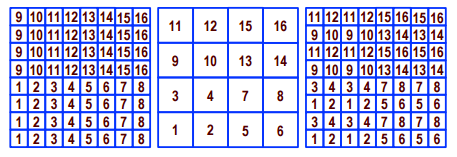
\includegraphics[scale = 1]{Partitioning.png}
\captionof{figure}{Three different partitioning schemes in 2D, from left to right: hybrid KBA, volumetric non-overloaded, and volumetric overloaded.}
\label{partitioning}
\end{minipage}

The overloaded volumetric partitioning proceeds as follows:

\begin{enumerate}
\item In a 2D (3D) domain, cellsets are divided into 4 (8) spatial quadrants (octants), with an equal number of cellsets in each  SQO (SQO is defined as a spatial quadrant or octant).
\item Assign 1/4 of the processors (1/8) in 3D to each SQO. 
\item Choose the individual overload factors $\omega_x, \omega_y, and \omega_z$ and individual processor counts $P_x, P_y, and P_z$, such that $\omega_x \omega_y \omega_z = \omega_r$ and $P_x P_y P_z = P$, with all $P_u$ even. $\omega_u$ is defined as the number of cellsets assigned to each $P_u$.
\item An array of $\omega_x\cdot\omega_y\cdot\omega_z$ ``tiles'' in each SQO. Each tile is an array of $1/2 P_x \cdot 1/2 P_y \cdot 1/2 P_z$ cellsets. These cellsets are mapped one-to-one to the $1/2 P_x \cdot 1/2 P_y \cdot 1/2 P_z$ procesors assigned to the SQO, using the same mapping in each tile.
\end{enumerate}
Each tile has a logically identical layout of cellsets, and each processor owns exactly one cellset in each tile in its SQO, making each processor responsible for $\omega_r$ cellsets.

The optimal scheduling algorithm rules are as follows:
\begin{enumerate}
\item If $i \leq X$, then tasks with $\Omega_x > 0$ have priority, while for $i > X$, tasks with $\Omega_x < 0$ have priority.
\item If multiple ready tasks have the same sign on $\Omega_x$, apply rule 1 to $j,Y,\Omega_y$.
\item If multiple ready tasks have the same sign on $\Omega_x$ and $\Omega_y$, apply rule 1 to $k,Z, \Omega_z$. 
\item If multiple tasks are ready in the same octant, then priority goes to the cellset for which the priority octant has greatest downstream depth.
\item If multiple ready tasks are in the same octant and have the same downstream depth of graph in $x$, then priority goes to the cellset for which the priority octant has greatest downstream depth of graph in $y$.
\item If multiple ready tasks are in the same octant and have the same downstream depth of graph in $x$ and $y$, then priority goes to the cellset for which priority octant has greatest depth of graph in $z$.
\end{enumerate}
This ensures that each SQO orders the octants: the one it can start right away ($A$), three that have one sign difference from$ A (B,C,$ and $D)$, three that have two sign differences ($\bar D, \bar C, \bar B$), and one in opposition to its primary ($\bar A$).

There are three constraints in order to achieve the optimal stage count. In these constraints, $M = \omega_g \omega_m/8$, which is the number of tasks per octant per cellset.
\begin{enumerate}
\item $ M \geq 2(Z-1)$
\item $\omega_z M \geq 2(Y-1)$
\item If $\omega_x > 1$, then $\omega_y \omega_z M \geq X$
\end{enumerate}
These conditions ensure there are no idle time in a variety of situations. At large processor counts, the product $\omega_m \omega_g$ must be large. This means that a weak scaling series refined only in space, but only coarsely refined in angle and energy, will eventually fail the constraints.

The optimal efficiency formula changes slightly from the KBA and hybrid KBA partitioning method in order to account for the overload factors. The only change is in the $\frac{N_{idle}}{N_{tasks}}$ term, as shown in Eq. \ref{overloadpartitioning}.
\begin{equation}
\varepsilon_{opt} = \frac{1}{[1+\frac{P_x+P_y+P_z-6}{\omega_g \omega_m \omega_r}][1+\frac{T_{\text{comm}}}{T_{\text{task}}}]}
\label{overloadpartitioning}
\end{equation}

\subsection*{KBA Partitioning}

Several parallel transport sweep codes use KBA partitioning in their sweeping, such as Denovo \cite{denovo} and PARTISAN\cite{partisan}.

The KBA algorithm traditionally chooses $P_z = 1, A_m = 1, G = A_g = 1, A_x = N_x/P_x, A_y = N_y/P_y$, with $A_z$ being the selectable number of z-planes to be aggregated into each task. With $N_k = N_z/A_z$, each processor performs $N_{\text{tasks}} = 8MN_k$ tasks. With the KBA algorithm, $2MN_k$ are pipelined from a given corner of the 2D processor layout. The far corner processor remains idle for the first $P_x + P_y - 2 $ stages, which means that a 2 octant sweep completes in $2MN_K + P_x + P_y - 2$ stages. If an octant-pair sweep does not begin until the previous pair's finishes, the full sweep requires $8MN_k + 4(P_x+P_y-2)$ stages, which means the KBA parallel efficiency is:
\begin{equation}
\varepsilon_{KBA} = \frac{1}{[1+\frac{4(P_x+P_y-2)}{8MN_k}][1+\frac{T_{\text{comm}}}{T_{\text{task}}}]}
\label{eKBA}
\end{equation}

%%%%%%%%%%%%%%%%%%%%%%%%%%%%%%%%%%%%%%%%%%
\subsection*{The Unstructured Transport Sweep}
%%%%%%%%%%%%%%%%%%%%%%%%%%%%%%%%%%%%%%%%%%

\tcr{avoid repeats from intro}


While PDT has scaled well out to 750,000 cores, similar levels of parallel scaling have not been achieved using unstructured sweeps yet. As described by Dr. Shawn Pautz \cite{Pautz}, a new list scheduling algorithm has been constructed for modest levels of parallelism (up to 126 processors).

There are three requirements for a sweep scheduling algorithm to have. First, the algorithm should have low complexity, since millions of individual tasks are swept over in a typical problem. Second, the algorithm should schedule on a set of processors that is small in comparison to the number of tasks in the sweep graph. Last, the algorithm should distribute work in the spatial dimension only, so that there is no need to communicate during the calculation of the scattering source. 

Here is the pseudocode for the algorithm:

\begin{verbatim}
Assign priorities to every cell-angle pair
Place all initially ready tasks in priority queue
While (uncompleted tasks)
    For i=1,maxCellsPerStep
       Perform task at top of priority queue
       Place new on-processor tasks in queue
    Send new partition boundary data
    Receive new partition boundary data
    Place new tasks in queue 
\end{verbatim}

An important part of the algorithm above is the assigning priorities to tasks. Specialized prioritization heuristics generate partition boundary data as rapidly as possible in order to minimize the processor idle time. 

Nearly linear speedups were obtained on up to 126 processors. Further work is being done for scaling to thousands of processors. 

\subsubsection{Cycle Detection}

\tcr{I do not understand the purpose of this section here}

A cycle is a loop in a directed graph. These occur commonly in unstructred meshes. The problem with cycles is that they can cause hang time in the problem, as a processor will wait for a message that might will never come. This means that the computation for one or more elements will never be completed. The solution to this is to ``break'' any cycles that exist by removing an edge of the task dependence graph (TDG). Old flux information is used on a particular element face in the domain. Most of the time, the edge removed is oriented obliquely with respect to the radiation direction. 

Algorithms for for finding cycles are called \textit{cycle detection} algorithms. This must be done efficiently in parallel, both because the task dependence graph is distributed, and because the finite element grid may be deforming every timestep and changing the associated TDG.

Cycle detection utilizes two operations: trim and mark. Trimming identifies and discards elements which are not in cycles. At the beginning of cycle detection, graphs are trimmied in the downwind direction, then the remaining graphs are trimmed in the upwind direction. A pivot vertex is then selected in each graph. Graph vertices are then marked as upwind, downwind, or unmarked. Then, if any vertices are both upwind and downwind, the cycle is these vertices plus the pivot vertex. An edge is removed between 2 cycle vertices, and 4 new graphs are created: a new cycle, the upwind vertices without the cycle, the downwind vertices without the cycle, and a set of unmarked vertices. This recursively continues until all cycles are eliminated.

\section{Motivation and Proposed Method for Load Balancing in PDT}

When discussing the parallel scaling of transport sweeps, a load balanced problem is of great importance. A load balanced problem has an equal number of degrees of freedom per processor. Load balancing is important in order to minimize idle time for all processors by equally distributing (as much as possible) the work each processor has to do.  For the purposes of unstructured meshes in PDT, we are looking to ``balance'' the number of cells. Ideally, each processor will be responsible for an equal number of cells. 

\tcr{input geometry : we are in the weeds here. Let's see the big picture first. unstructured grids -why are they useful, why do we want them? then how can we use unstructured grids, many people use tets, explain our logic, 2D unstructured triangular, excluded in 3rd D; then, maybe, you can explain that the 2D unstructured triangular grids will come from the use of the triangle mesh generator. The we can talk about 2D geometries being described using PSLG. But there is still no need to use the words input file.}

When using the unstructured meshing capability in PDT, the input geometry is described by a Planar Straight Line Graph (PSLG). This is a list of vertices and the straight line segments connecting them. The mesh generator being used is the Triangle Mesh Generator \ref{triangle}, so the PSLG input is described by a Triangle .poly file. In order to parallelize the sweep, the user determines how many ``subsets'', he/she would like to subdivide the PSLG into. A series of cut planes in $x$ and $y$ are laid over the PSLG, creating an overlaid regular Cartesian grid \tcr{would a graph be nice to illustrate this here?}. Each convex, orthogonal unit created by the grid is termed a ``subset''. Subsets then become the base structured unit when calculating our parallel efficiency. Subsets are created and meshed in parallel. Within each subset lies an unstructured triangular meshed. Discontinuities along the boundary are fixed by ``stitching'' across hanging nodes, creating degenerate polygons along subset boundaries. Because PDT's spatial discretization employs Piece-wise Linear Discontinuous (PWLD) finite element basis functions, there is no problem solving on degenerate polygons. 

If the number of cells in each subset can be reasonably balanced, then the problem is effectively load balanced. The Load Balance algorithm described on the next page details how the subsets will be load balanced. In summary, the procedure of the algorithm involves moving the initially user specified $x$ and $y$ cut planes, re-meshing, and iterating until a reasonably load balanced problem is obtained. 

\noindent\begin{minipage}{\textwidth}
\textbf{Load Balance:} A load balancing algorithm that equalizes the number of triangles per subset. \\
\rule{\textwidth}{0.4pt}
\begin{algorithmic}
\STATE  $I,J$ subsets specified by user

\STATE Mesh all subsets

\STATE  $N_{tot} = $ total number of triangles
\STATE  $N_{ij} = $ number of triangles in subset $ij$

\STATE $f =\underset{ij}{\text{max}}(N_{ij})/\frac{N_{tot}}{I\cdot J}$

\COMMENT {//Check if all subsets meet the tolerance}
\IF {$f < \text{tol}_{\text{subset}}$}
	\STATE DONE with load balancing
\ELSE
	\STATE $f_I = \underset{i}{\text{max}}[\sum_{j} N_{ij}]/\frac{N_{tot}}{I}$
	
	\STATE $f_J = \underset{j}{\text{max}}[\sum_{i} N_{ij}]/\frac{N_{tot}}{J}$
	
	\IF {$f_I > \text{tol}_{\text{row}}$}
		\STATE \textbf{Redistribute}($X_i$)
	\ENDIF
	
	\IF{$f_J > \text{tol}_{\text{col}}$}
		\STATE \textbf{Redistribute}($Y_j$)
	\ENDIF 
	
	\IF {redistribution occured}
		\STATE REMESH and repeat algorithm
	\ENDIF
	
\ENDIF

\IF {There is still a discrepancy amongst subsets}
     \STATE Move cutplane segments on the subset level and remesh (may require changes to scheduling algorithm)
\ENDIF
\end{algorithmic}
\rule{\textwidth}{0.4pt}
\end{minipage}

\bigskip

\noindent\begin{minipage}{\textwidth}
\textbf{Redistribute:} A function that moves cut lines in either X or Y. \\
\rule{\textwidth}{0.4pt}
\begin{algorithmic}
\STATE \textbf{Input:}CutLines (X or Y vector that stores cut lines). 
\STATE \textbf{Input:} num\_tri\_row or num\_tri\_col, a pArray containing number of triangles in each row or column 
\STATE \textbf{Input:} The total number of triangles in the domain, $N_{tot}$

\STATE stapl::array\_view num\_tri\_view, over num\_tri\_row/column
\STATE stapl::array\_vew offset\_view

\STATE stapl::partial\_sum(num\_tri\_view) \COMMENT {Perform prefix sum}

\COMMENT {We now have a cumulative distribution stored in offset\_view}

\FOR {$i = 1$ :CutLines.size()-1}

	\STATE vector <double> pt1 = [CutLines(i-1), offset\_view(i-1)]
	\STATE vector <double> pt2 = [CutLines(i), offset\_view(i)]
	\STATE ideal\_value = $i\cdot \frac{N_{tot}}{\text{CutLines.size()}-1}$
	\STATE X-intersect(pt1,pt2,ideal\_value) \COMMENT{Calculates the X-intersect of the line formed by pt1 and pt2 and the line y = ideal\_value.}
	\STATE CutLines(i) = X-intersect
\ENDFOR
\end{algorithmic}
\rule{\textwidth}{0.4pt}
\end{minipage}


\section{Preliminary Results}

Unstructured meshing capability has been placed in PDT, Figure coming to showcase it (probably C5G7 reactor mesh). 

\section{Goals and Proposed Plan}

%\subsection{Completed Work}
\begin{itemize}
\item Unstructured meshing capability in PDT for 2D and 2D extruded problems.\tcr{2D + 2D extruded}
\item {Unstructured meshing is generated in parallel using the same partitioning scheme and number of processors as the sweep.}
\item {Stitching between meshed subdomains to preserve interface continuity.}
%\end{itemize}

%\subsection{Planned Work}
%\begin{itemize}
\item Implement load balancing algorithm for unstructured meshes in PDT. A load balanced problem would be defined by $f$ in the pseudocode, or the subset with the maximum number of cells, divided by the average number of cells per subset.\tcr{Metric definition}
\item Code verification and testing to prove load balancing algorithm effectiveness. 
\item Results of the parallel transport sweeps for benchmark problems.
\end{itemize}

\tcr{possible outlook for the research}

\subsection{Possibly Outlook for Research}
\begin{itemize}
\item Propose a scaling study for unstructured meshes in PDT, similar to the infamous Zerr problem.
\end{itemize}

\bibliographystyle{plain}
\bibliography{./Proposal}

\end{document}